% !TEX encoding = UTF-8 Unicode
% !TEX root = thesis-ex.tex

\label{Sec:JetRec}
For the measurement presented here, we use the jets reconstructed in the calorimeter 
using the \antikt\ algorithm \cite{Cacciari:2008gp} with \RFour.
The underlying event (UE) contribution to jets is subtracted on 
an event by event basis at the cell level.
The details on the jet reconstruction 
procedure and performance in heavy ion collisions have been described in 
\cite{ATLAS-COM-PHYS-2011-1733}, here we will only shortly summarize the main 
features of the heavy ion jet reconstruction.

In order to reconstruct jets in heavy ion collisions, a large background from 
the UE has to be subtracted from each jet.

The UE subtraction procedure is done in several iterative steps.

First an estimate of the UE average transverse energy density, $\rho_i(\eta)$, 
is evaluated for each calorimeter layer $i$ in intervals of $\eta$ of width 
$\Delta \eta = 0.1$ using all cells in each calorimeter layer, within a given 
$\eta$ interval excluding those within $\Delta R < 0.4$ of ``seed'' jets.
In the first 
subtraction step, the ``seed'' jets are defined to be jets reconstructed using the 
\antikt\ algorithm with \RTwo\ jets which have at 
least one tower  (a tower is a 0.1x0.1 region of the calorimeter and the energy
associated with it is the sum of the energies from all contributing calorimeter layers
in that region)
with $\Et > 3$~GeV and which have a ratio of the maximum to 
the mean tower associated with the jet of at least 4.

  The UE-subtracted cell energies  were calculated according to:
\begin{equation}
\label{eqn:UE}
E_{\mathrm{T},i}(\eta, \phi)^{\mathrm{sub}} = E_{\mathrm{T},i}(\eta, \phi) - A_i \times \rho_i(\eta) 
\end{equation}
where $E_{\mathrm{T},i}$, $\eta$, $\phi$,  and $A_i$ represent the $\Et$, $\eta$, 
$\phi$, and area of the cell in the layer $i$.
The $\rho_i(\eta)$ is the energy density per unit area in the layer $i$.
The kinematics for \RTwo\ jets 
generated in this first subtraction step were calculated via a four-vector sum 
of all (assumed massless) cells contained within the jets using the \Et\ values 
obtained from Eq.~\ref{eqn:UE}.

The second subtraction step starts with the definition of a new set of 
seeds using a list of \RTwo\ calorimeter jets from the first 
subtraction step, each with $\Et > 4$~GeV.
Using this new set of 
seeds, a new estimate of the UE, $\rho'_i(\eta)$, was calculated excluding 
cells within $\Delta R < 0.4$ of the new ``seed'' jets, where $\Delta R = \sqrt{ 
(\eta_{\mathrm{cell}} - \eta_{\mathrm{jet}})^2 + (\phi_{\mathrm{cell}} - \phi_{\mathrm{jet}})^2}$.


The jet energy scale calibration is based on the numerical inversion method and provides calibration constants for all jet collections used in this study~\cite{HICalib}.
The final jet energy calibration using in-situ studies is applied in the offline analysis and it is described in Sec~\ref{Sec:JetSelection}.
  



The jet reconstruction performance in 5.02 TeV \pp\ collisions was evaluated using corresponding MC samples with a full detector simulation.
The kinematics of the truth jets are reconstructed from primary particles\footnote{Primary particles are defined as having a mean lifetime of $\tau > 0.3 \times 10^{-10}$ s, and are produced directly in \pp\ interactions or from decays of particles with shorter lifetimes} with the \antikt\ algorithm with radius parameter $R = 0.4$.
The jet reconstruction efficiency, JES (in this case evaluated as $\langle (\ETreco)\rangle/\ETtrue$), and JER for \pp\ collisions is shown in Fig.~\ref{Fig:Performancepp5} for \RFour\ jet.
For \pbpb\ collisions the JES is shown in Fig.~\ref{Fig:PerformancepbpbJES} and the JER is shown
in Figure~\ref{Fig:PerformancepbpbJER}.
 Further studies of the jet performance in the 2015 \pbpb\
data are found in Ref.~\cite{Aad:2014bxa}.
Figures~\ref{Fig:PerformancepbpbJPReta0p4}-\ref{Fig:PerformancepbpbJPRphi0p4} present the jet angular resolution in $\eta$ and $\phi$ as a function of jet \pt\ evaluated in six centrality classes.
The angular resolution is improving with the increasing jet \pT\ and decreasing collision centrality.
The angular resolution is found to be significantly better for smaller jets as expected since the smaller jets are less affected by the presence of the UE.


\begin{figure}
\centerline{
\begin{tabular}{cc}
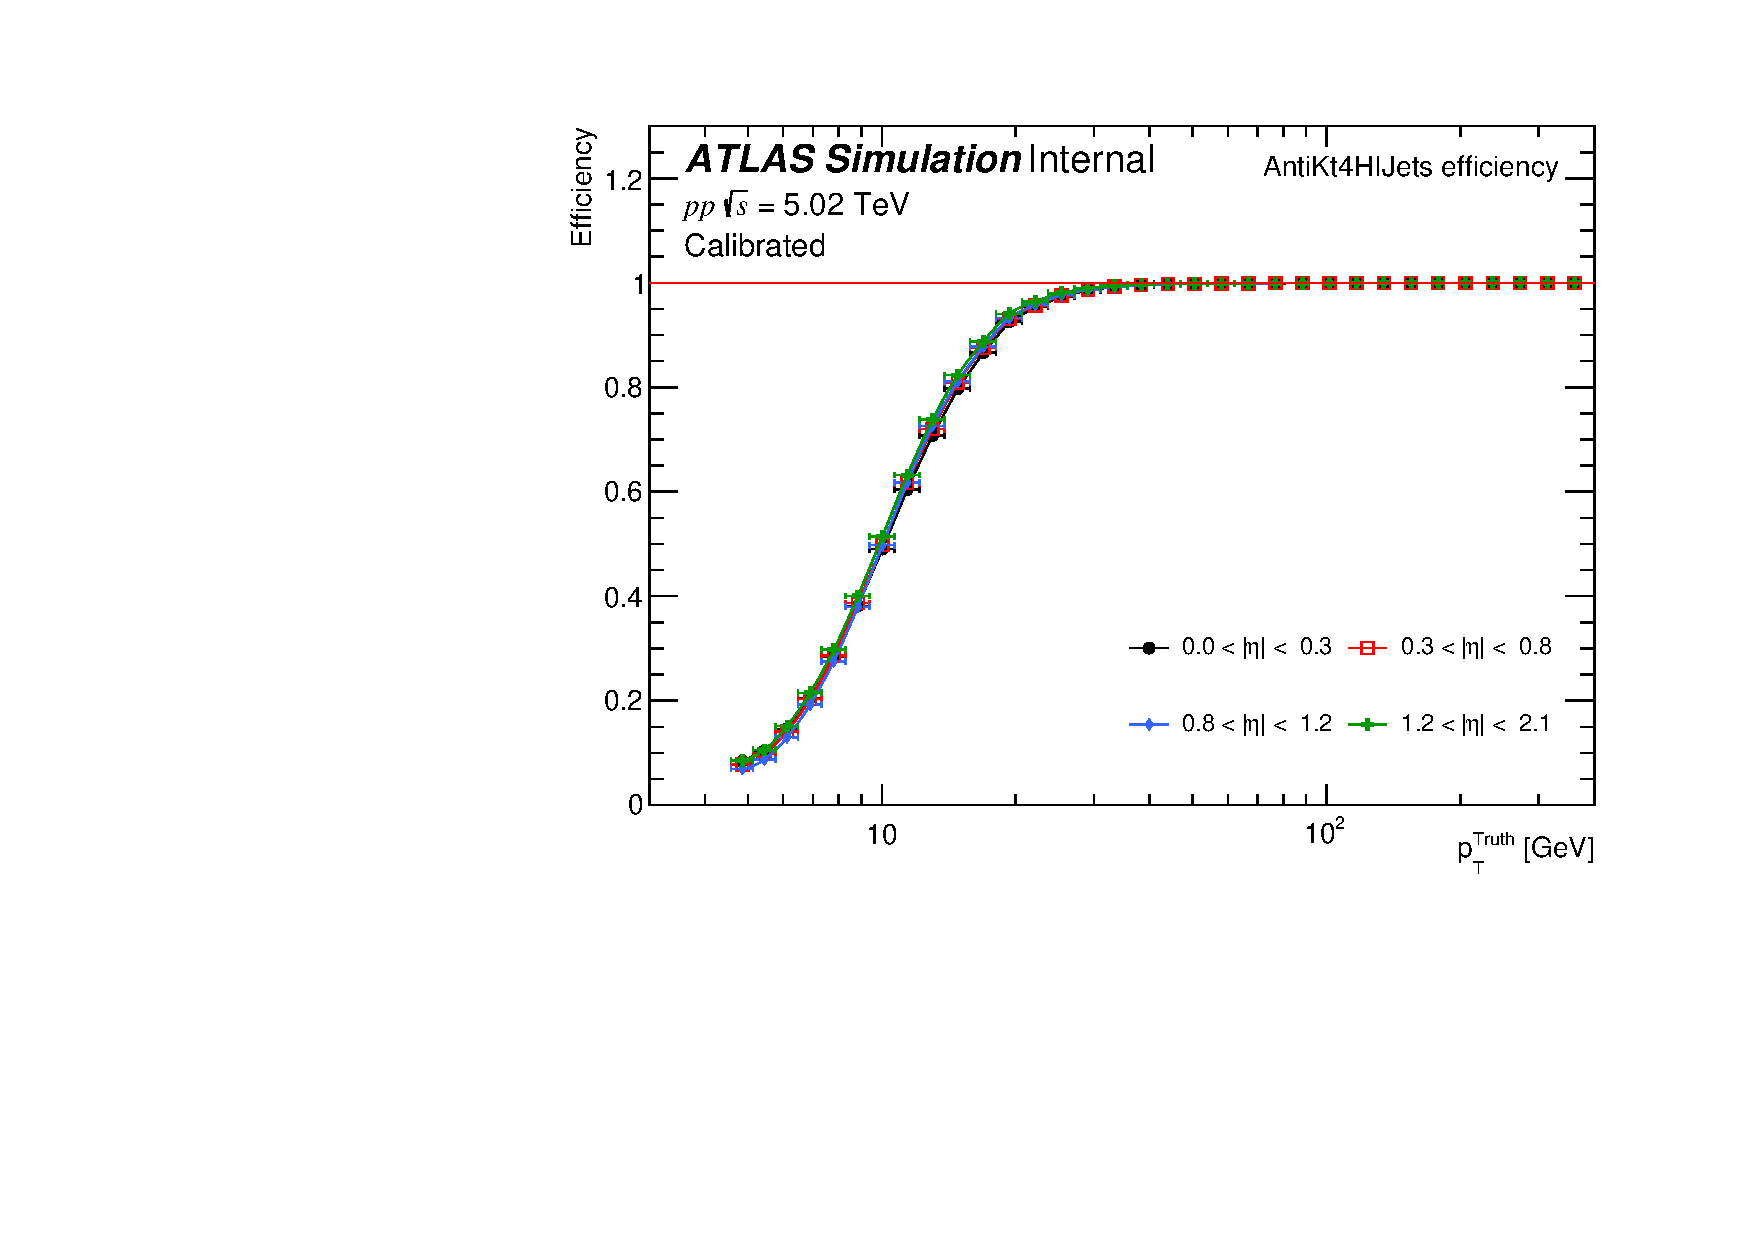
\includegraphics[width=7cm]{figures/main/general/Eff_pp5.pdf} &
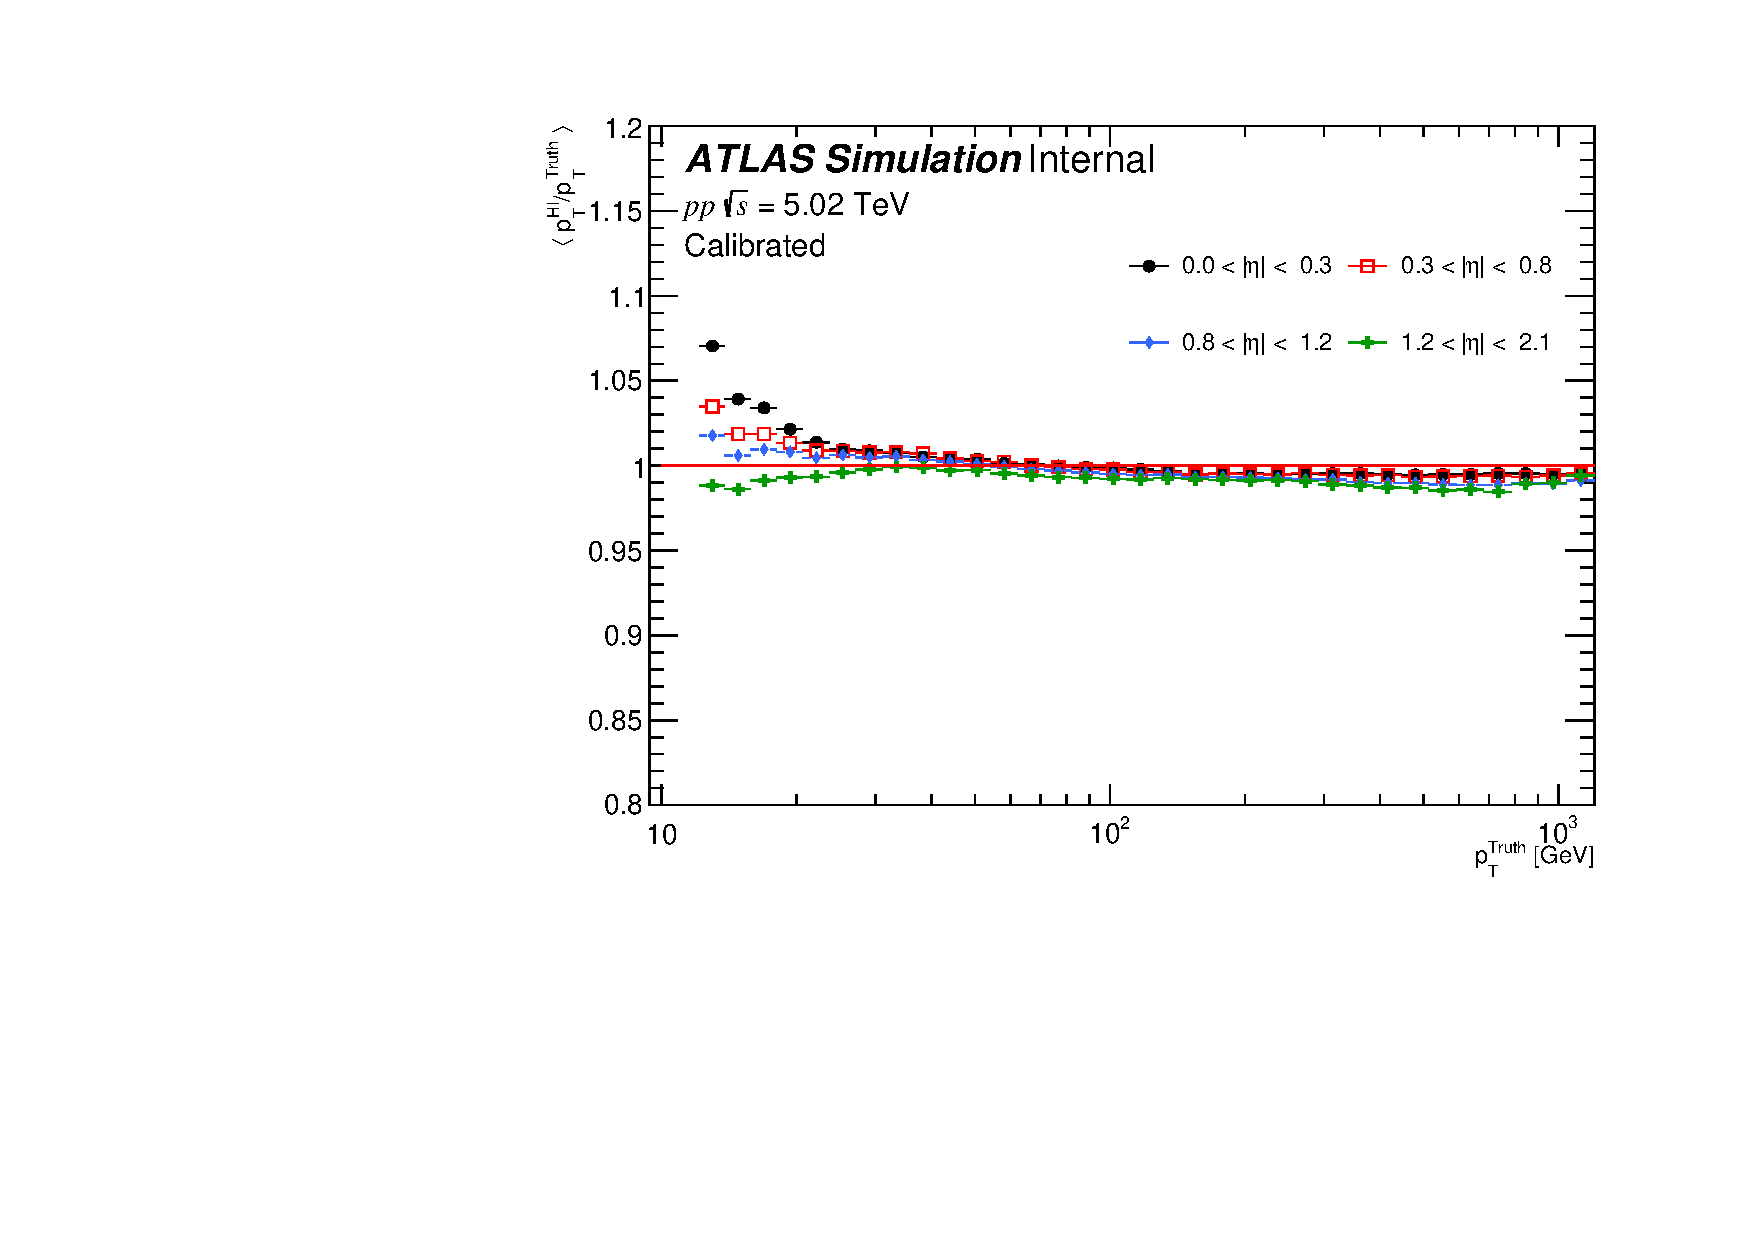
\includegraphics[width=7.3cm]{figures/main/general/JES_pp5.pdf} \\
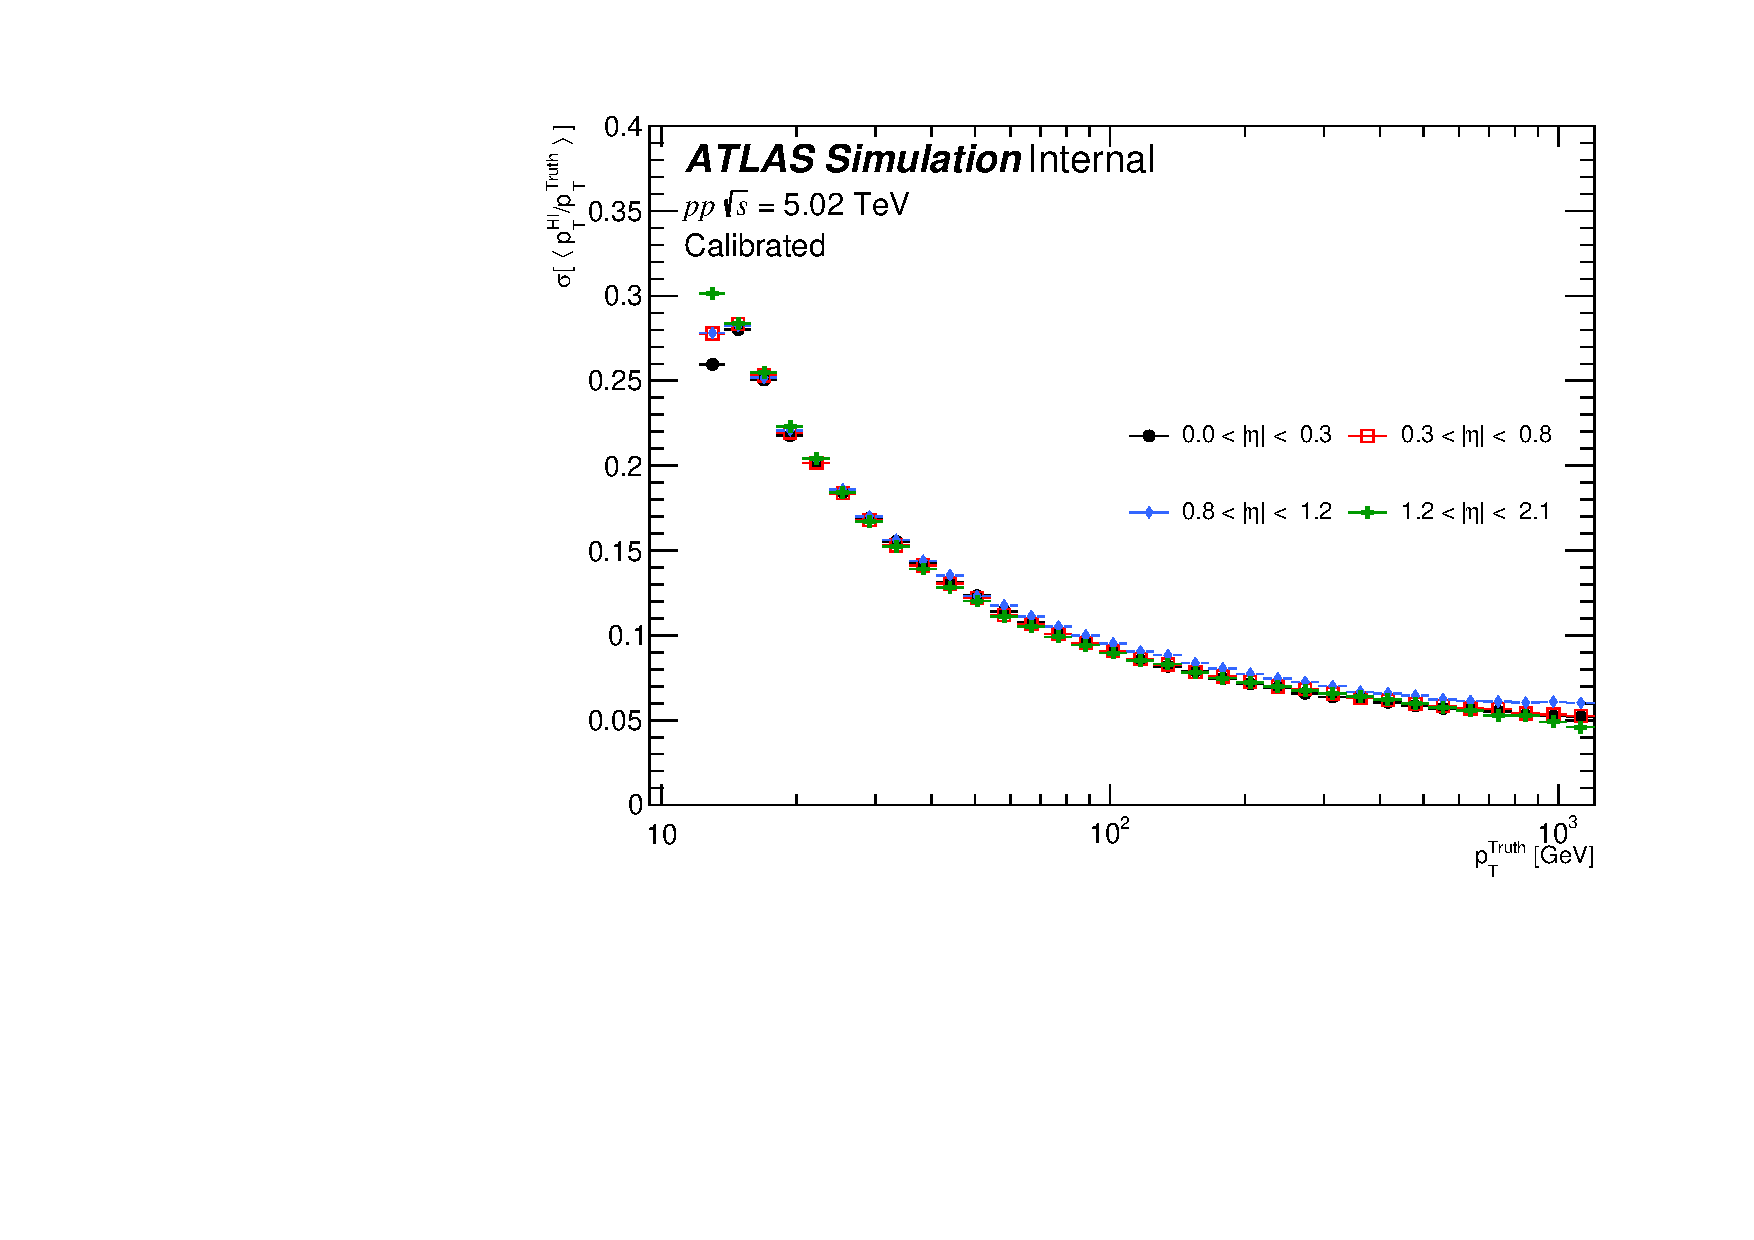
\includegraphics[width=7.3cm]{figures/main/general/JER_pp5.pdf} 
\end{tabular}}
\caption{
Top panels: Jet reconstruction efficiency in 5.02 TeV \pp\ collisions (left) as a function of truth jet \pT\ and different $\eta$ bins.
Jet energy scale (JES) in 5.02 TeV \pp\ collisions (right) as a function of truth jet \pT\ and different $\eta$ bins.
Bottom panels: Jet energy resolution (JER) in 5.02 \pp\ collisions as a function of truth jet \pT\ and different $\eta$ bins.
}
\label{Fig:Performancepp5}
\end{figure}

\begin{figure}
   \centering
   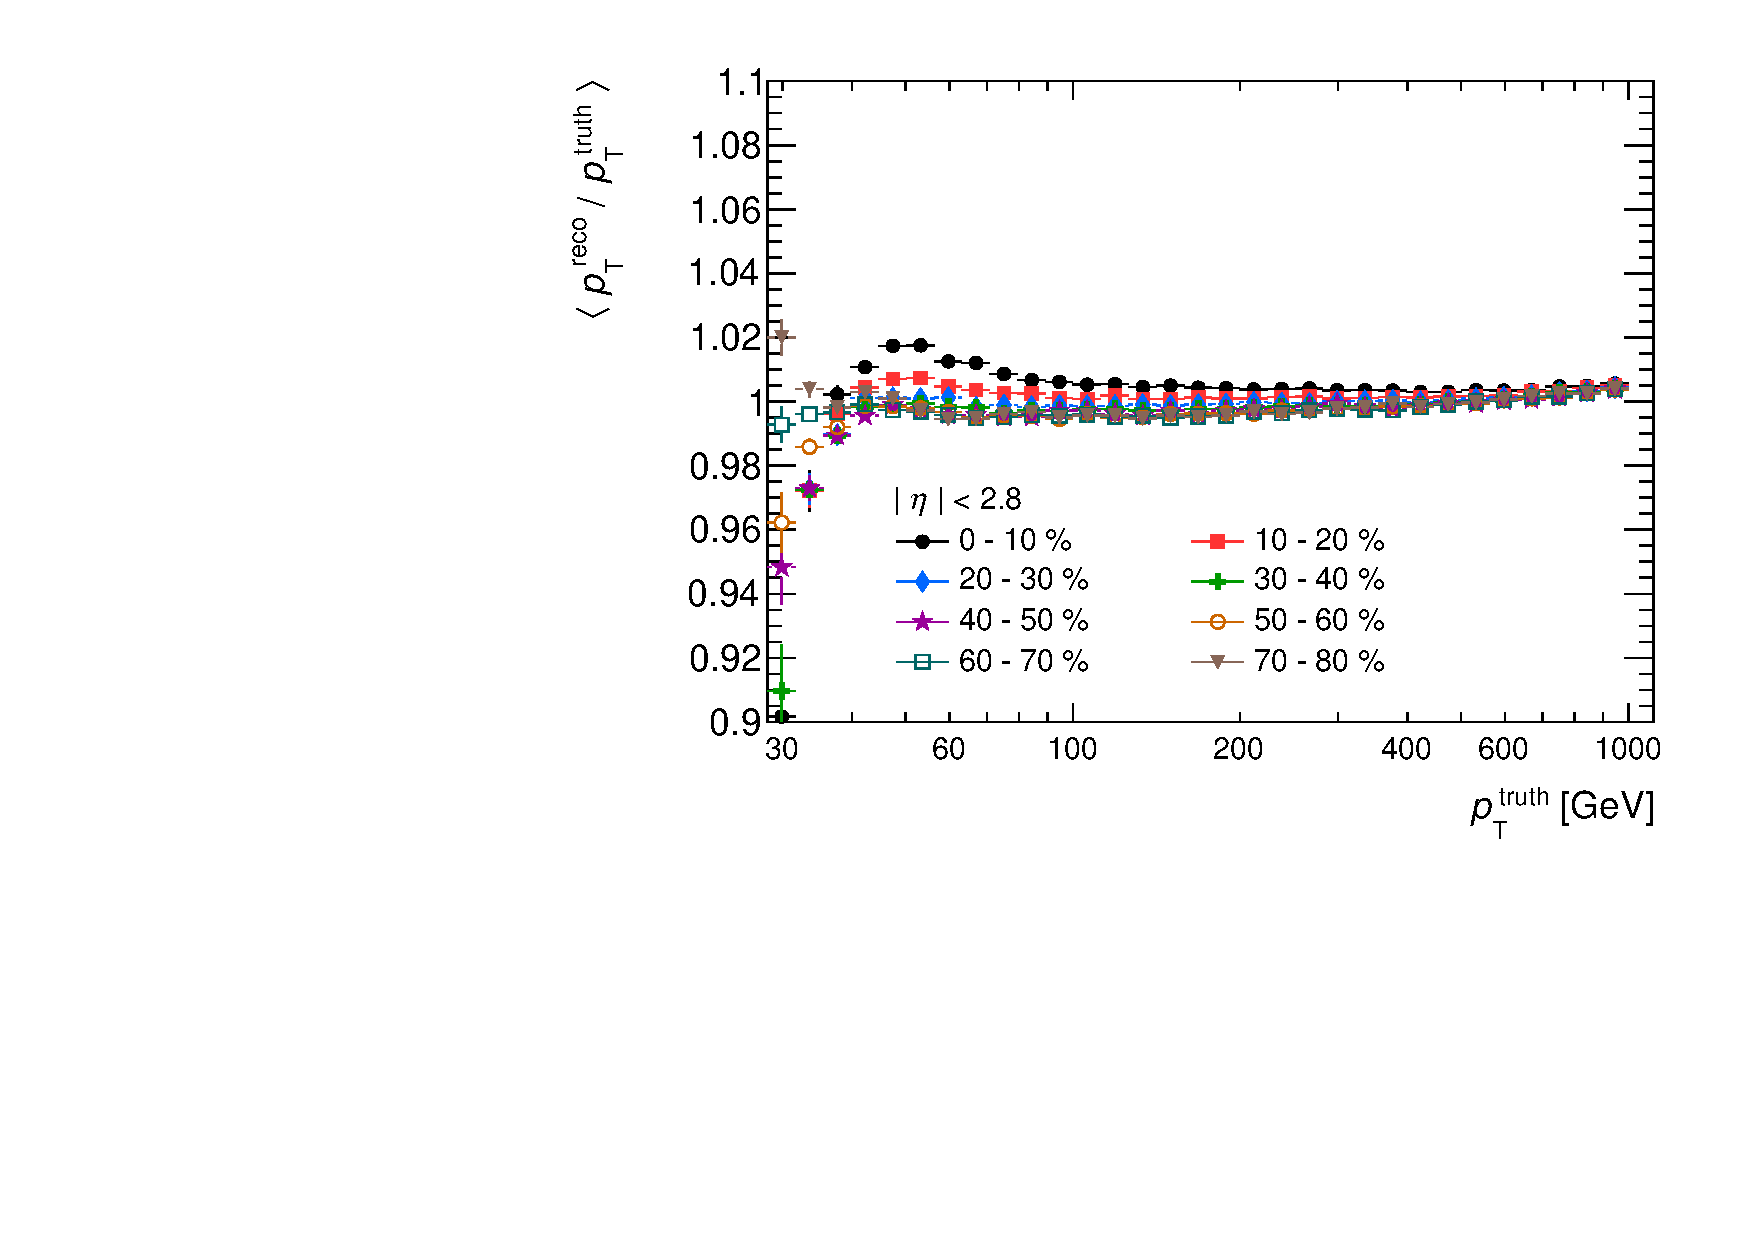
\includegraphics[width = 0.75\textwidth]{figures/main/general/PbPb_JES_pT_eta2p8.pdf}
   \caption{ JES in \pbpb\ collisions for eight centrality selections.
 Plot is from Ref.~\cite{Aad:2014bxa}.}
   \label{Fig:PerformancepbpbJES}
\end{figure}

\begin{figure}
   \centering
   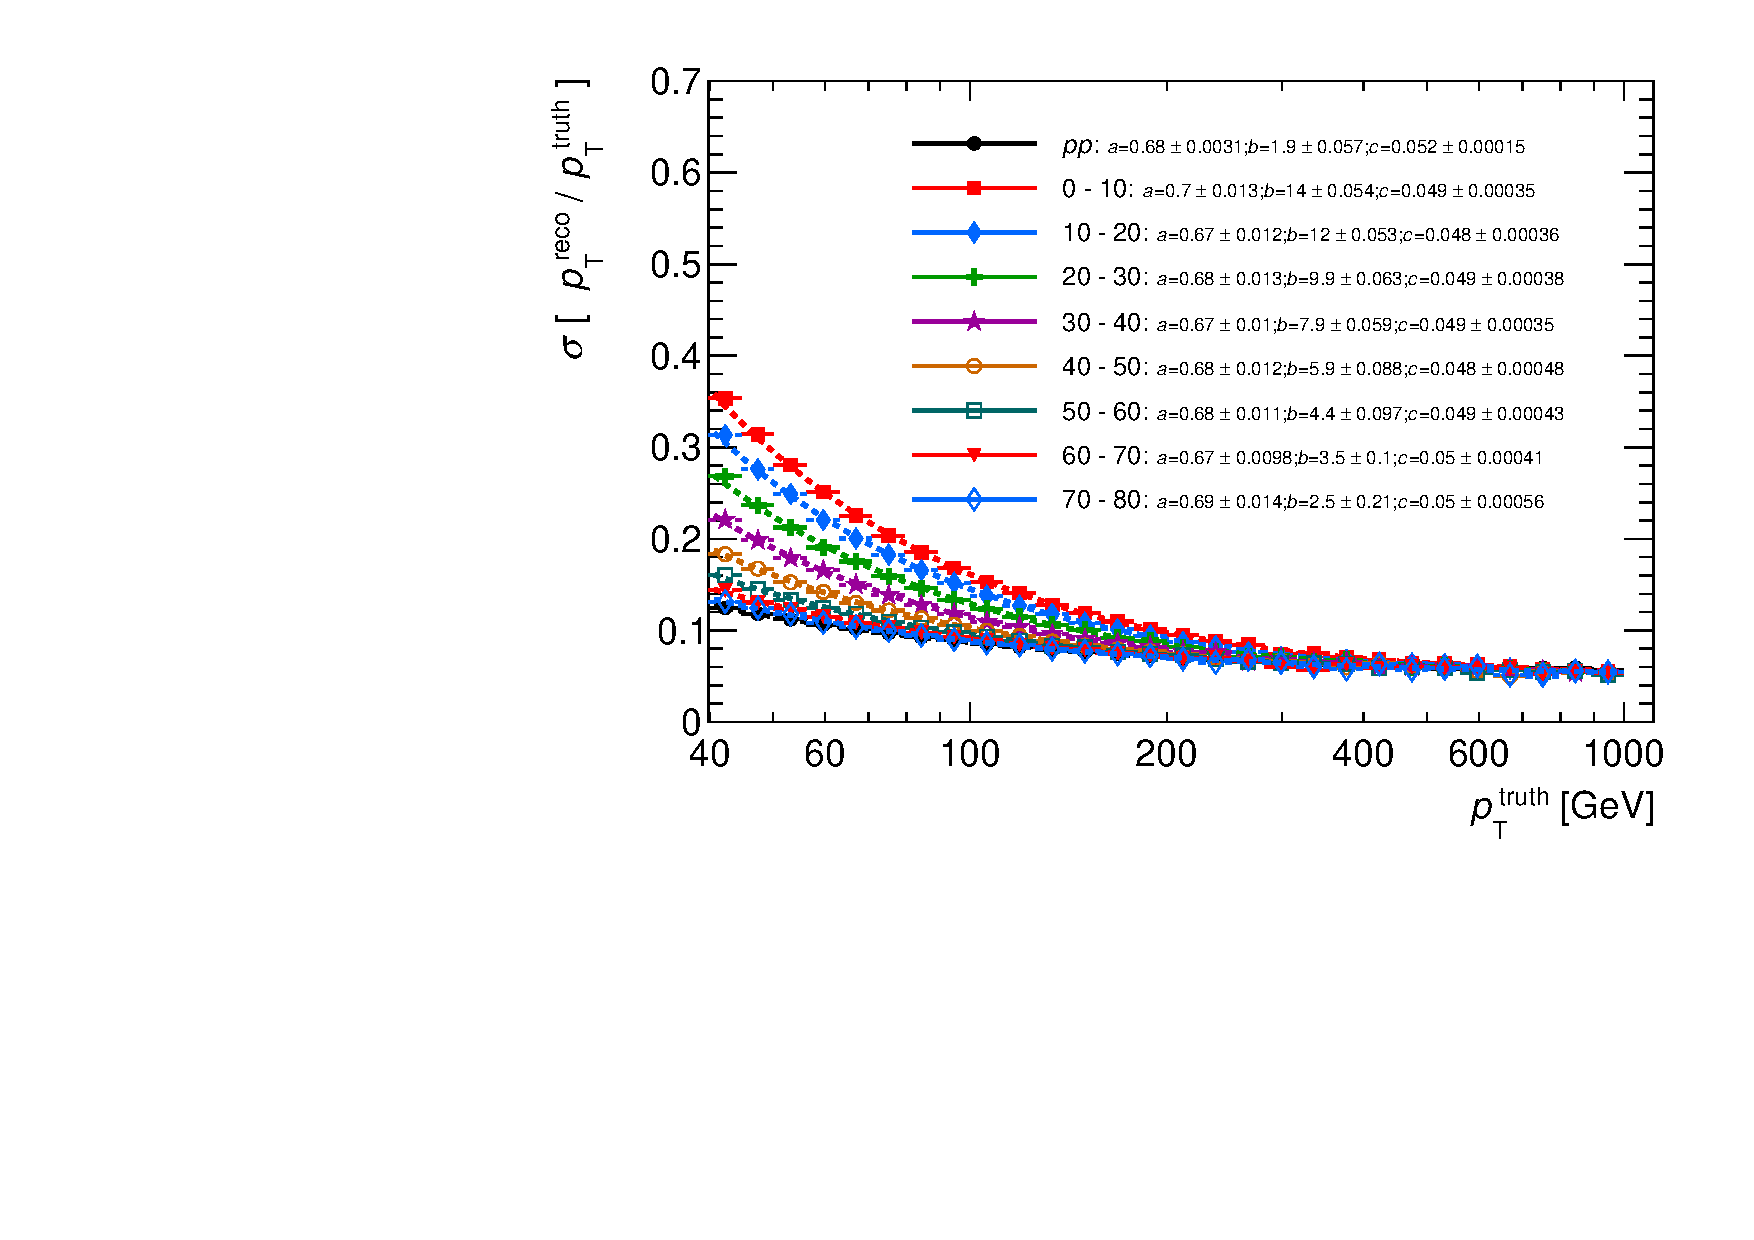
\includegraphics[width = 0.75\textwidth]{figures/main/general/PbPb_JER_pT_eta2p8.pdf}
   \caption{ JER in \pbpb\ collisions for eight centrality selections.
 Plot is from Ref.~\cite{Aad:2014bxa}.
The points are fit to the standard function that describes the calorimetric resolution.}
   \label{Fig:PerformancepbpbJER}
\end{figure}


\begin{figure}
   \centering
   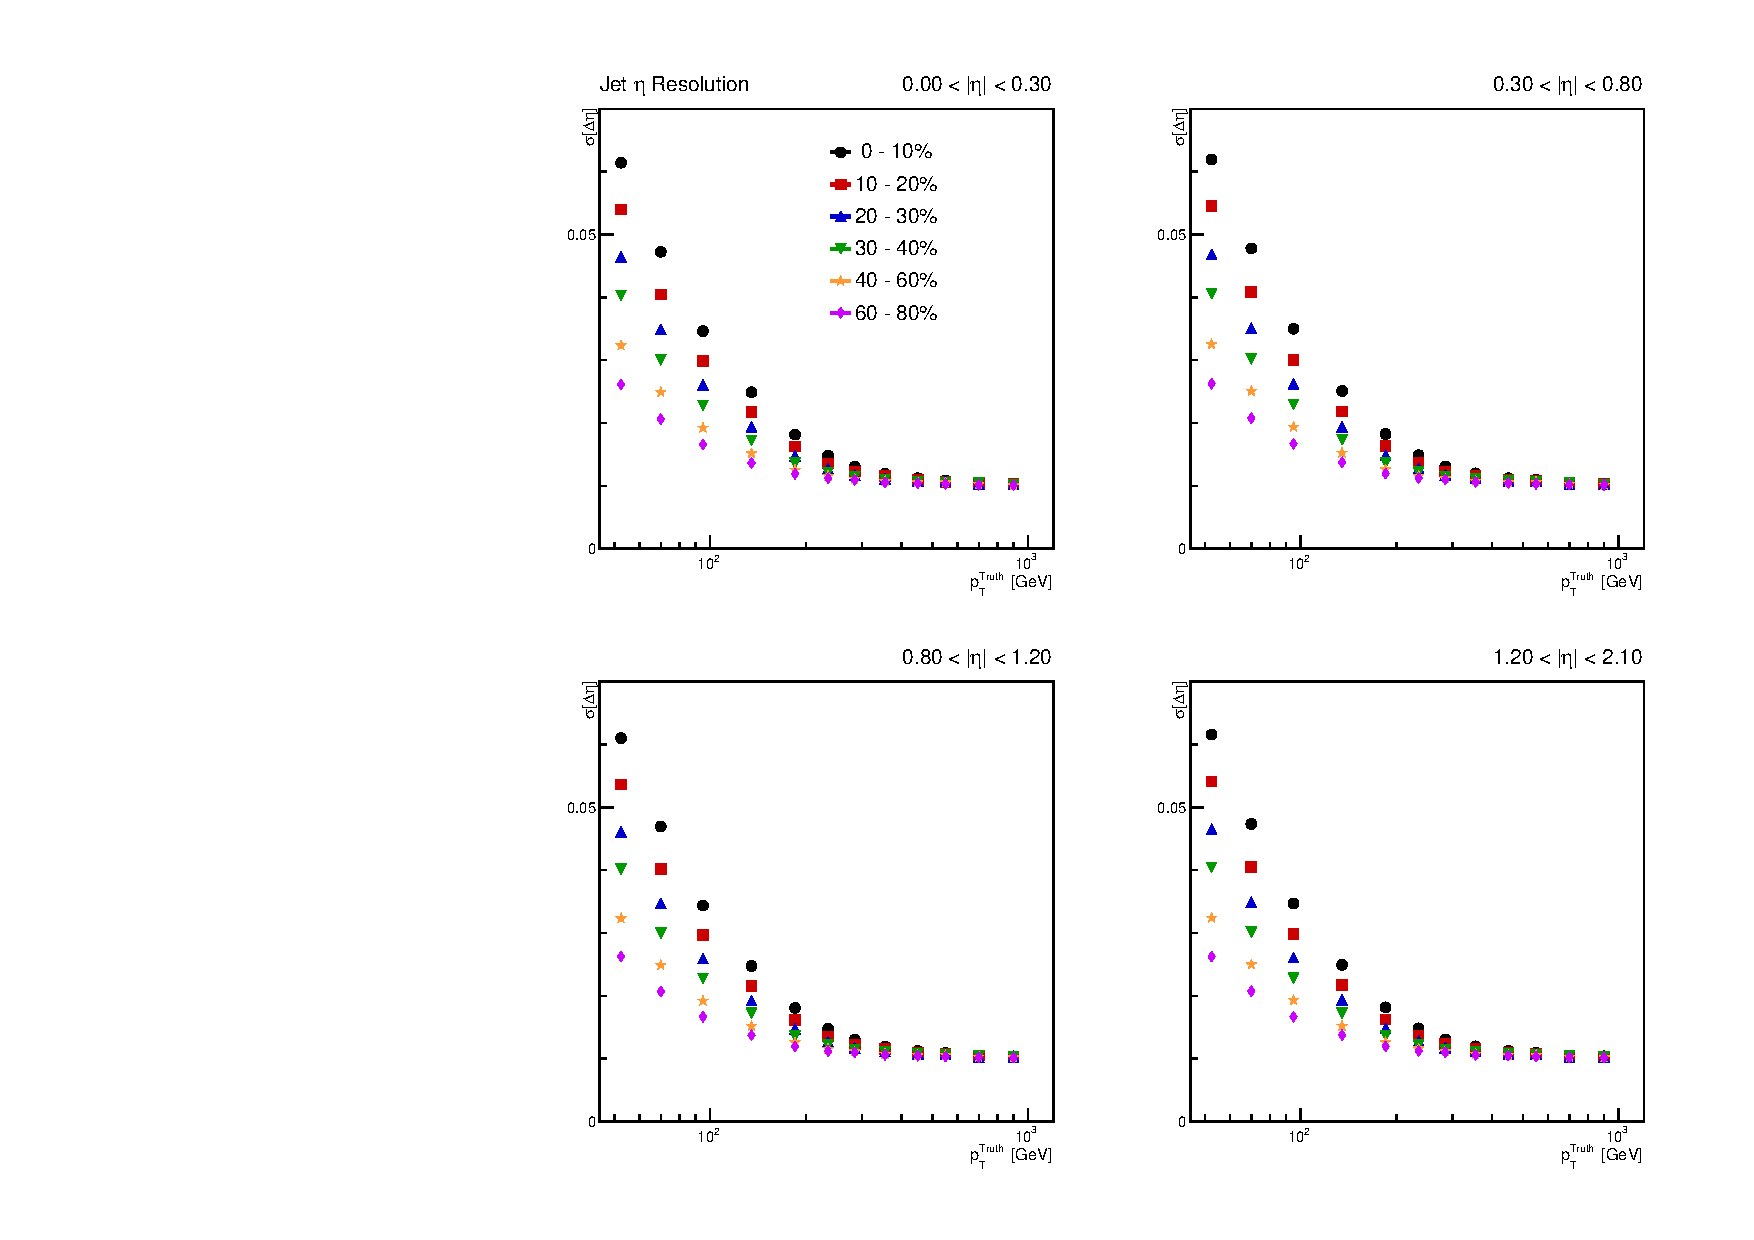
\includegraphics[width = 0.75\textwidth]{figures/main/general/jet_res_eta_r04.pdf}
   \caption{ Jet angular resolution in $\eta$ for $R=0.4$ jets in \pbpb\ collisions as a function of jet \pT\ for six centrality selections.}
   \label{Fig:PerformancepbpbJPReta0p4}
\end{figure}

\begin{figure}
   \centering
   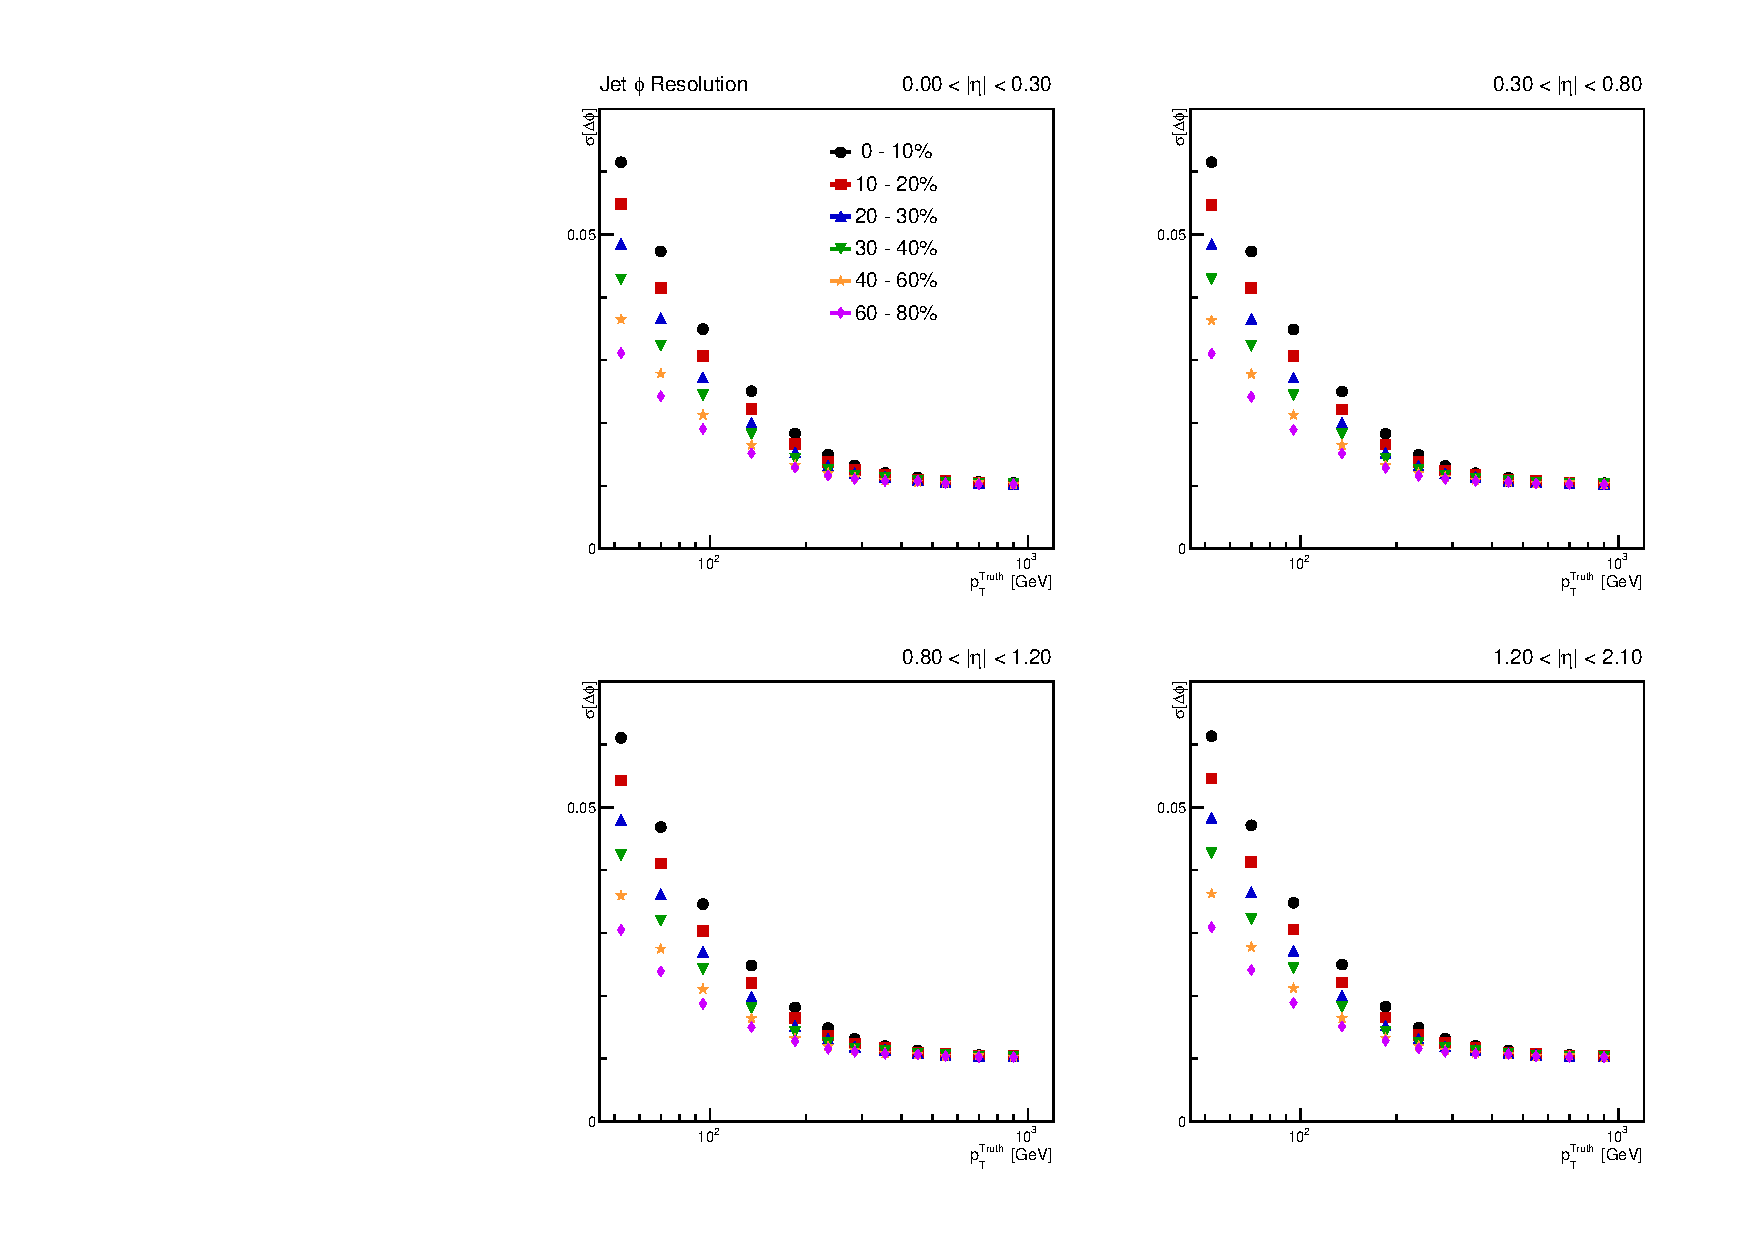
\includegraphics[width = 0.75\textwidth]{figures/main/general/jet_res_phi_r04.pdf}
   \caption{ Jet angular resolution in $\phi$ for $R=0.4$ jets in \pbpb\ collisions as a function of jet \pT\ for six centrality selections.}
   \label{Fig:PerformancepbpbJPRphi0p4}
\end{figure}

